%!TEX root = ../main.tex
\section{Basic Model under Risk}
\begin{frame}\begin{center}
\LARGE\textbf{Basic Model under Risk}
\end{center}\end{frame}
%-------------------------------------------------------------------------------
%-------------------------------------------------------------------------------
\begin{frame}
\textbf{Ingredients}\medskip
\begin{itemize}\setlength\itemsep{1em}
\item Objectives
\item Constraints\medskip
\begin{itemize}\setlength\itemsep{1em}
\item Institutions
\item Information
\end{itemize}
\end{itemize}
\vspace{0.3cm}\hspace{0.3cm}$\Rightarrow$ Optimal Decision
\end{frame}

%-------------------------------------------------------------------------------
%-------------------------------------------------------------------------------
\begin{frame}
\textbf{Notation}
\begin{align*}\begin{array}{ll}
k = 1, \hdots, K 				&  \text{Alternative}\\
t = 1, \hdots, T	&  \text{Time}\\
S(t)	&  \text{State Space at Time $t$}\\
R_k(S(t),t)  &  \text{Rewards for Alternative $k$ at Time $t$}\\
d_k(t)  &  \text{Indicator for Alternative $k$ at Time $t$}\\
\delta  & \text{Discount Factor}
\end{array}\end{align*}
\end{frame}
%-------------------------------------------------------------------------------
%-------------------------------------------------------------------------------
\begin{frame}
\begin{center} \textbf{Decision Tree}\\\vspace{0.5cm}
\scalebox{0.8}{\begin{tikzpicture}
  [
    grow                    = right,
    sibling distance        = 6em,
    level distance          = 10em,
    edge from parent/.style = {draw, -latex},
    every node/.style       = {font=\footnotesize, minimum width={width("Magnetometer")+2pt}},
    sloped
  ]
  \node [root] {Start}
    child { node [env] {Home}}
    child { node [env] {School}}
    child { node [env] {Occupation B}
            child { node [env] {Home}} 
            child { node [env] {School}}
            child { node [env] {Occupation B}}
            child { node [env] {Occupation A}}
           }
    child { node [env] {Occupation A}};
\end{tikzpicture}}
\end{center}
\end{frame}
%-------------------------------------------------------------------------------
%-------------------------------------------------------------------------------
\begin{frame}
\begin{center} \textbf{Timing of Events}\vspace{0.9cm}
\scalebox{0.9}{	%!TEX root = ../main.tex
	\begin{tikzpicture}[scale=1.0, every node/.style={scale=0.8}]

	\tikzset{
	eqblock/.style={text width=3cm,align=center}
	}

	% Nodes
	\node (left) {};
	\node[below right=3cm and 1cm of left] (bottom_left) {};
	\node[node distance=12cm, right of=left] (right) {};
	\node[node distance=12cm, right of=bottom_left] (bottom_right) {};

	\node[node distance=6cm, right of=left, yshift=-.5cm] (t1) {\large$t$};
	\node[node distance=6cm, right of=bottom_left, yshift=-.5cm] (t2) {\large$t+1$};

	\node[eqblock, above of=left, xshift=3cm] (eq1) {\large$R_k(S(t),t)$};
	\node[eqblock, above of=left, xshift=6cm] (eq2) {\large$d_k(t)$};
	\node[eqblock, above of=left, xshift=9cm] (eq3) {\large$R_k(S(t),t)$};
	\node[eqblock, above of=bottom_left, xshift=3cm] (eq4) {\large$R_k(S(t+1),t+1)$};
	\node[eqblock, above of=bottom_left, xshift=6cm] (eq6) {\large$d_k(t+1)$};
	\node[eqblock, above of=bottom_left, xshift=9cm] (eq5) {\large$R_k(S(t+1),t+1)$};

	\node[above of=eq1, node distance=1cm] (text2) {\large Learn};
	\node[above of=eq2, node distance=1cm] (text3) {\large Choose};
	\node[above of=eq3, node distance=1cm] (text1) {\large Receive};
	\node[above of=eq4, node distance=1cm] (text4) {\large Learn};
	\node[above of=eq6, node distance=1cm] (text5) {\large Choose};
	\node[above of=eq5, node distance=1cm] (text6) {\large Receive};

	% Lines
	\draw[|-|] (left) -- (right);
	\draw[|-|] (bottom_left.center) -- (bottom_right);

	\end{tikzpicture}
}
\end{center}
\end{frame}
%-------------------------------------------------------------------------------
%-------------------------------------------------------------------------------
\begin{frame}
\textbf{Agents' Objective under Risk}\vspace{0.3cm}
\begin{align*}
V(S(t),t) = \max_{\{d_k(t)\}_{k \in K}} E\left[ \sum_{\tau = t}^T \delta^{\tau - t} \sum_{k\in K}R_k(\tau)d_k(\tau)\Bigg| S(t)\right]\\
\end{align*}
\end{frame}
%-------------------------------------------------------------------------------
%-------------------------------------------------------------------------------
\begin{frame}
\textbf{Bellman Equations}\vspace{0.3cm}
\begin{align*}
V(S(t),t) = \max_{k \in K}\{V_k(S(t),t)\},
\end{align*}
where for all but the final period:
\begin{align*}
V_k(S(t),t) = R_k(S(t),t) + \delta E\left[V(S(t + 1), t + 1)\mid S(t), d_k(t) = 1\right]
\end{align*}
\end{frame}
%-------------------------------------------------------------------------------
%-------------------------------------------------------------------------------
\subsection{Calibrated Example}
\begin{frame}\begin{center}
\LARGE\textit{Calibrated Example}
\end{center}\end{frame}
%-------------------------------------------------------------------------------
%-------------------------------------------------------------------------------
\begin{frame}
\textbf{Agent Characteristics}\vspace{0.3cm}
\begin{align*}\begin{array}{ll}
x_{1,t} &  \text{Experience in Occupation A at Time $t$}\\
x_{2,t} &  \text{Experience in Occupation B at Time $t$}\\
s_{t}  &  \text{Years of Schooling at Time $t$}
\end{array}\end{align*}
\end{frame}
%-------------------------------------------------------------------------------
%-------------------------------------------------------------------------------
\begin{frame}\vspace{0.3cm}

\textbf{Occupation A}\vspace{0.3cm}
\begin{align*}
R_1(t) & = \exp\{\alpha_{10} + \alpha_{11}s_t + \alpha_{12}x_{1,t} - \alpha_{13}x_{1,t}^2 + \alpha_{14}x_{2,t} - \alpha_{15}x_{2,t}^2 + \epsilon_{1,t}  \}
\end{align*}\vspace{-1.2cm}

\begin{center}
\begin{tabular}{L{1.8cm} C{1cm} C{1cm} C{1cm} C{1.2cm} C{1cm} C{1cm}}\toprule
Parameters  &  $\alpha_{10}$ &  $\alpha_{11}$ &  $\alpha_{12}$ &  $\alpha_{13}$ &  $\alpha_{14}$ &  $\alpha_{15}$ \\\midrule
    Values  &  9.21 & 0.04 &  0.033 &  0.0005  &  0.00 &  0.00\\\bottomrule
\end{tabular}
\end{center}


\end{frame}
%-------------------------------------------------------------------------------
%-------------------------------------------------------------------------------
\begin{frame}\vspace{0.3cm}

\textbf{Occupation B}\vspace{0.3cm}
\begin{align*}
R_2(t) & = \exp\{\alpha_{20} + \alpha_{21}s_t + \alpha_{22}x_{1,t} - \alpha_{23}x_{1,t}^2 + \alpha_{24}x_{2,t} - \alpha_{25}x_{2,t}^2 + \epsilon_{2,t}  \}
\end{align*}\vspace{-1.2cm}


\begin{center}
\begin{tabular}{L{1.8cm} C{1cm} C{1cm} C{1cm} C{1.2cm} C{1cm} C{1cm}}\toprule
Parameters  &  $\alpha_{20}$ &  $\alpha_{21}$ &  $\alpha_{22}$ &  $\alpha_{23}$ &  $\alpha_{24}$ &  $\alpha_{25}$ \\\midrule
    Values  &  8.20& 0.08&  0.022 &  0.0005  &  0.067 &  0.001\\\bottomrule
\end{tabular}
\end{center}


\end{frame}

%-------------------------------------------------------------------------------
%-------------------------------------------------------------------------------
\begin{frame}
\begin{center}\textbf{Wages and Experience}\vspace{-0.5cm}
\begin{figure}[h!]\centering
\subfloat[Occupation A]{
\scalebox{0.35}{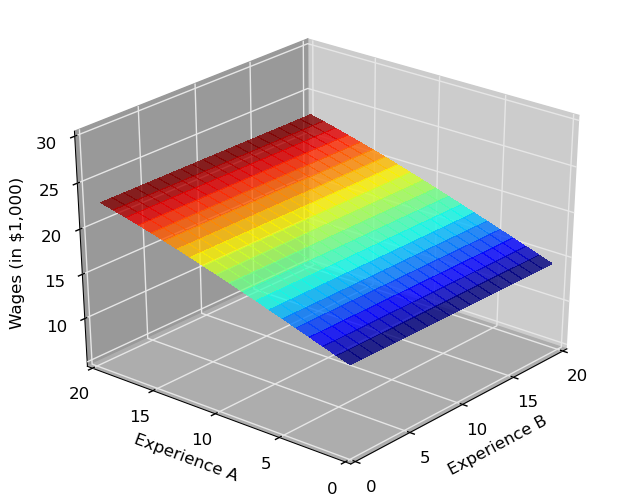
\includegraphics{../material/returns_experience_a}}}
\subfloat[Occupation B]{\
\scalebox{0.35}{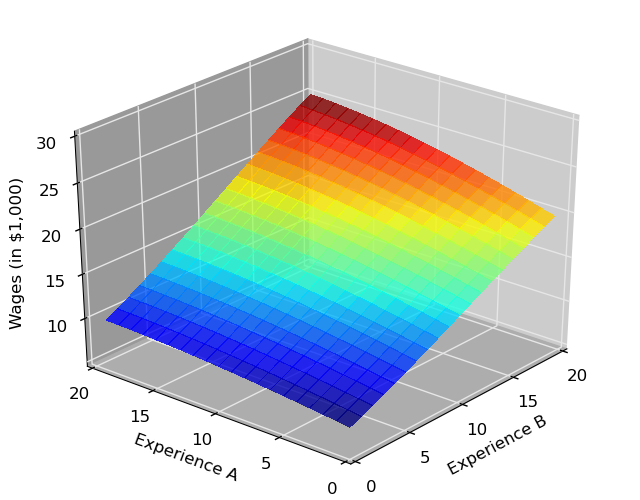
\includegraphics{../material/returns_experience_b}}}
\end{figure}\end{center}\end{frame}

%-------------------------------------------------------------------------------
%-------------------------------------------------------------------------------
\begin{frame}
\begin{center} \textbf{Wages and Schooling}\vspace{0.3cm}
\scalebox{0.40}{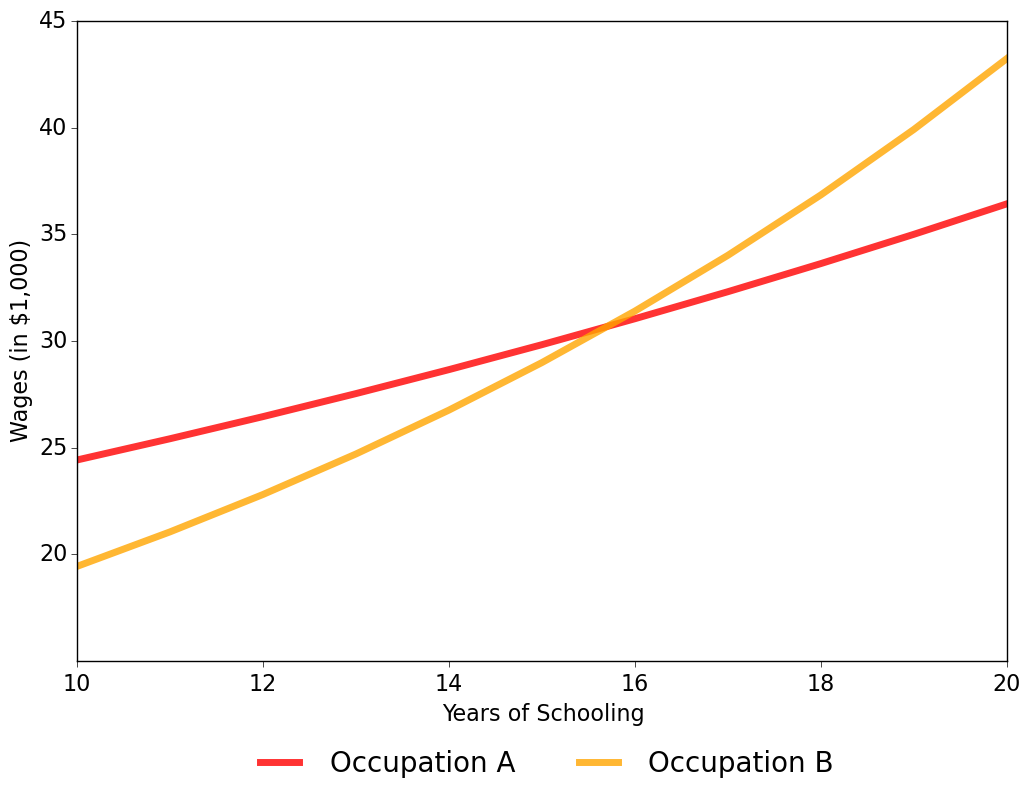
\includegraphics{../material/returns_schooling}}
\end{center}\end{frame}

%-------------------------------------------------------------------------------
%-------------------------------------------------------------------------------
\begin{frame}\vspace{0.3cm}

\textbf{School}\vspace{0.3cm}
\begin{align*}
R_3(t) & = \underbrace{\left(\beta_0 - \beta_1(1 - d_3(t - 1))\right)}_{\text{Psychic Costs}} - \beta_2\Ind\left[s_t \geq 13 \right] + \epsilon_{3,t}
\end{align*}\vspace{-0.5cm}

\begin{center}
\begin{tabular}{L{1.8cm} C{1.2cm} C{1.2cm} C{1.2cm}}\toprule
     Parameters  &  $\beta_{0}$ &  $\beta_{1}$ &  $\beta_{2}$ \\\midrule
     Values  &  5,000  & 15,000 &  5,000 \\\bottomrule
\end{tabular}
\end{center}


\end{frame}
%-------------------------------------------------------------------------------
%-------------------------------------------------------------------------------
\begin{frame}\vspace{0.3cm}

\textbf{Home}\vspace{0.3cm}
\begin{align*}
R_4(t) & = \gamma_0 + \epsilon_{4,t}
\end{align*}\vspace{-0.5cm}

\begin{center}
\begin{tabular}{L{1.8cm} C{1.1cm}}\toprule
     Parameter &  $\gamma_0$ \\\midrule
     Value      &  14,500     \\\bottomrule
\end{tabular}
\end{center}

\end{frame}
%-------------------------------------------------------------------------------
%-------------------------------------------------------------------------------
\begin{frame}
\textbf{State Space}\vspace{0.3cm}
\begin{itemize}
\item at time $t$
\begin{align*}
S(t) & = \{s_t, x_{1,t}, x_{2,t}, d_3(t-1), \epsilon_{1,t}, \epsilon_{2,t}, \epsilon_{3,t}, \epsilon_{4,t}\}
\end{align*}
\item laws of motion
\begin{align*}
x_{j, t + 1} & = x_{j, t} + d_j(t) & \forall\quad j \in \{1, 2\}  \\[1em]
s_{t + 1}    & = s_t + d_3(t) &  \\[1em]
f(\epsilon_{t + 1}\mid S(t), d_k(t)) & = f(\epsilon_{t + 1}\mid \bar{S}(t), d_k(t))
\end{align*}
\end{itemize}
\end{frame}
%-------------------------------------------------------------------------------
%-------------------------------------------------------------------------------
\begin{frame}
\textbf{Shocks}\vspace{0.3cm}

\scriptsize\begin{eqnarray*}
\begin{pmatrix}
\epsilon_{1,t}\\
\epsilon_{2,t}\\
\epsilon_{3,t}\\
\epsilon_{4,t}
\end{pmatrix} & \sim & \mathcal{N}_0\left[\left(\begin{array}{c}
0\\
0\\
0\\
0
\end{array}\right),\left(\begin{array}{cccc}
16\times10^{-4}  &   0.00              &   0.00  &     0.00 \\
0.00            &   25\times10^{-2} &    0.00   &    0.00 \\
0.00            &   0.00              & 36\times10^{6}   &    0.00 \\
0.00            &   0.00              &   0.00 & 36\times10^{6}
\end{array}\right)\right]
\end{eqnarray*}

\end{frame}
%-------------------------------------------------------------------------------
%-------------------------------------------------------------------------------
\begin{frame}
\begin{center}\textbf{Choices over Time}\vspace{0.3cm}
\scalebox{0.40}{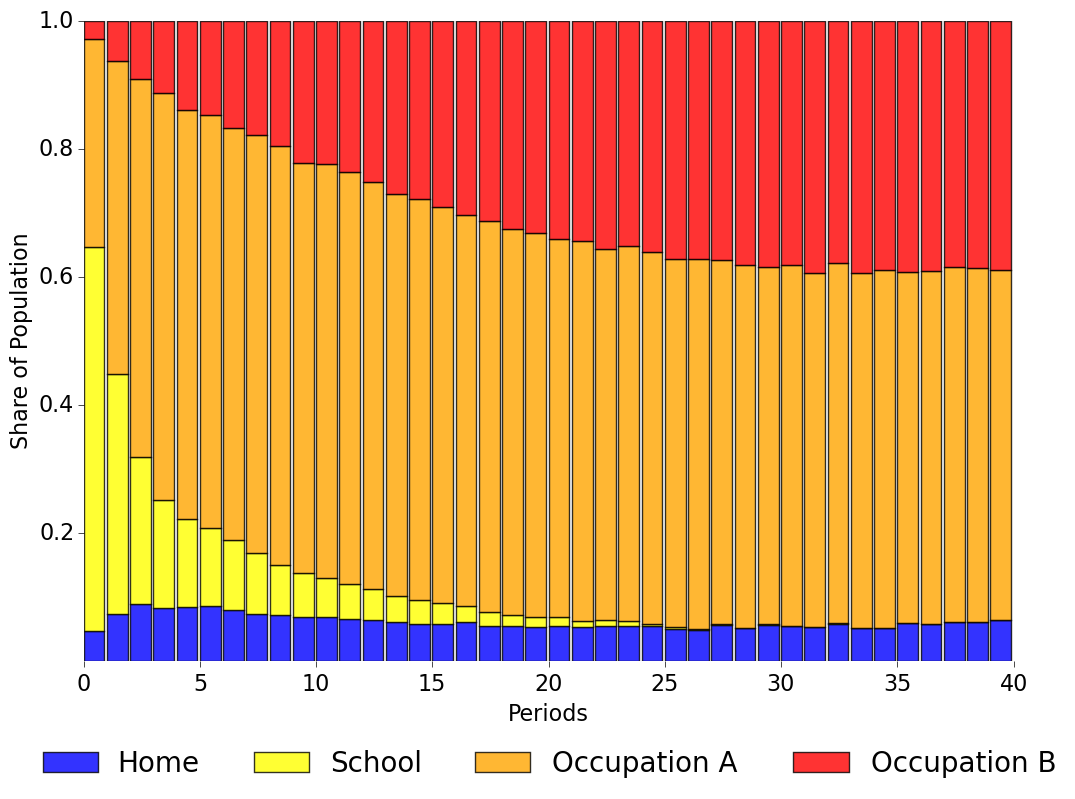
\includegraphics{../material/choice_patterns_0000}}
\end{center}\end{frame}
